\documentclass{article}
\usepackage[utf8]{inputenc}
\usepackage{CJKutf8}
\usepackage{amsmath}
\usepackage{amsfonts}
\usepackage{amssymb}
\usepackage{graphicx}
\usepackage{float}
% \usepackage{geometry}
\usepackage{url}
% \geometry{a4paper, margin=1in}

% Define keywords command
\newcommand{\keywords}[1]{\textbf{关键词:} #1}

\title{基于混合 ResNet-ComplexCNN 与高斯过程回归去噪的增强型自动调制分类方法}
\author{某某某}
\date{2025年6月}

\begin{document}
\begin{CJK}{UTF8}{gbsn}

\maketitle

\begin{center}
    \textbf{浙江工业大学} \\
    \textbf{机器学习大作业} \\
    \textbf{题目: 基于混合 ResNet-ComplexCNN 与高斯过程回归去噪的增强型自动调制分类方法} \\
    \vspace{0.5cm}
    \begin{tabular}{|l|l|}
        \hline
        学院: & 信息工程学院 \\
        \hline
        专业: & 智能科学与技术 \\
        \hline
        班级: & 智能科学与技术实验班 \\
        \hline
        学号: & \\
        \hline
        学生姓名: & 某某某 \\
        \hline
        指导老师: & 导师姓名及职称 \\
        \hline
        提交日期: & 2025年6月 \\
        \hline
    \end{tabular}
\end{center}

\newpage
\begin{abstract}
自动调制分类(AMC)作为无线通信智能化的关键技术,在频谱感知、信号监测和认知无线电等领域具有重要意义。随着5G/6G通信系统的快速发展和频谱资源日益稀缺,准确识别不同调制方式对于优化频谱利用率、提高通信质量和增强网络安全性至关重要。本文提出了一种基于RML2016.10a数据集的增强型自动调制分类方法,解决了现有深度学习方法在强噪声环境下分类准确率下降的关键问题。

我们设计了一种创新的混合神经网络架构,将ResNet的残差学习能力与 Complex CNN的复数信号处理优势相结合,并融入高斯过程回归(GPR)进行自适应噪声降低。该方法的核心创新包括:(1)基于信噪比自适应的GPR去噪算法,通过精确的噪声标准差估计和自适应长度尺度调整,实现不同SNR条件下的最优去噪效果;(2)利用调制信号星座图旋转对称性设计的数据增强策略,对训练信号进行$90^{\circ}$、$180^{\circ}$、$270^{\circ}$旋转变换,显著提升模型的泛化能力;(3)混合 ComplexResNet 架构,通过复数残差块直接处理 I/Q 信号的实部和虚部,结合残差连接机制有效缓解梯度消失问题,实现快速收敛和优异性能。

实验结果表明,所提出的方法在RML2016.10a 数据集上达到了65.38\%的分类准确率,相比现有最先进方法取得了显著提升。消融研究验证了三重改进策略的有效性: GPR 去噪、旋转数据增强和混合架构分别贡献了不同程度的性能提升。本研究为复杂电磁环境下的调制识别提供了新的解决方案,对推动认知无线电和智能通信系统的发展具有重要价值。

代码已开源至: \url{https://github.com/LJK666666666/radioML-v3}

\end{abstract}

\keywords{自动调制分类, 深度学习, ResNet, 复数神经网络, 高斯过程回归, 信号去噪, 数据增强}

\newpage
\begin{abstract}
Automatic modulation classification (AMC), as a key technology for intelligent wireless communications, is of great significance in the fields of spectrum sensing, signal monitoring and cognitive radio. With the rapid development of 5G/6G communication systems and the increasing scarcity of spectrum resources, accurate identification of different modulation modes is crucial for optimizing spectrum utilization, improving communication quality and enhancing network security. In this paper, we propose an enhanced automatic modulation classification method based on the RML2016.10a dataset, which solves the key problem of degradation of classification accuracy of existing deep learning methods in strong noise environments.

We design an innovative hybrid neural network architecture that combines the residual learning capability of ResNet with the complex signal processing advantages of ComplexCNN and incorporates Gaussian Process Regression (GPR) for adaptive noise reduction. The core innovations of the method include: (1) GPR denoising algorithm based on signal-to-noise ratio (SNR) adaptation, which realizes the optimal denoising effect under different SNR conditions through accurate noise standard deviation estimation and adaptive length scale adjustment; (2) data enhancement strategy designed by utilizing the rotational symmetry of the constellation diagram of the modulated signals, which rotates and transforms the training signals by $90^{\circ}$, $180^{\circ}$, and $270^{\circ}$ to significantly improve the model's generalization ability; (3) hybrid ComplexResNet architecture, which directly processes the real and imaginary parts of the I/Q signals through complex residual blocks, combined with the residual connection mechanism to effectively mitigate the gradient vanishing problem and achieve fast convergence and excellent performance.

Experimental results show that the proposed method achieves a classification accuracy of 65.38\% on the RML2016.10a dataset, which is a significant improvement over existing state-of-the-art methods. The ablation study validates the effectiveness of the triple improvement strategy: the GPR denoising, rotated data enhancement, and hybrid architecture contribute to different degrees of performance improvement, respectively. This study provides a new solution for modulation identification in complex electromagnetic environments, which is valuable for advancing the development of cognitive radio and intelligent communication systems.

The code has been open-sourced to: \url{https://github.com/LJK666666666/radioML-v3}

\keywords{automatic modulation classification, deep learning, ResNet, complex neural networks, Gaussian process regression, signal denoising, data enhancement}
\end{abstract}

\newpage
\tableofcontents

\newpage
\section{绪论}

\subsection{研究背景}
在现代无线通信系统中,自动调制识别(Automatic Modulation Recognition, AMR)作为频谱感知、干扰检测和非协作通信等功能的核心技术,承担着对未知信号进行实时分类的任务。随着无线电环境的日益复杂,信号在传播过程中往往会遭遇多径衰落、载波频偏以及强噪声干扰等非理想因素,使得传统基于手工设计特征(如高阶累积量、循环谱等)加以机器学习分类的方法在低信噪比(SNR)和恶劣信道条件下识别性能急剧下降,难以满足实际系统的需求。

近年来,深度学习技术凭借端到端学习的能力和对高维特征的自动提取优势,迅速成为AMR研究的主流方向。其中,卷积神经网络(CNN)通过多层卷积层和池化层,能够有效捕捉信号的局部时频特征;而长短期记忆网络(LSTM)则通过循环结构擅长处理序列数据,能够建模信号的长期依赖性。

尽管如此,现有方法仍面临诸多挑战:首先,单一网络结构往往在某些调制类型或信道条件下表现优异,却难以在全谱段范围内保持稳定———过拟合高SNR数据或难以泛化到低 SNR 场景;其次,大多数深度模型以实数运算为主,无法直接利用I/Q信号中的相位信息,导致复杂信号特征难以充分挖掘;此外,为了提升准确率而堆叠的深层网络往往带来巨大的计算和存储开销,不利于资源受限的终端设备部署。

因此,在保持高识别精度的同时,如何设计既能兼顾不同信道条件下的鲁棒性、充分利用复数信号本征特性,又能满足计算效率和部署成本约束的AMR框架,成为业界和学术界亟待解决的重要课题。

\subsection{研究意义}
自动调制识别(AMR)作为现代通信系统中的一项基础性和关键性技术,在无线电频谱监测、干扰识别、非合作通信识别、认知无线电等领域都发挥着不可替代的作用。然而,目前的AMR技术距离实际通信环境中的实际需求仍有一定差距。本研究的意义主要体现在以下几个方面:

\begin{enumerate}
    \item 增强复杂通信环境下的系统鲁棒性 \\
    现实中的无线通信环境通常具有多径衰落、频率偏移和干扰信号等多种复杂因素,单一模型或方法在实际应用场景中往往难以兼顾不同环境条件下的准确性和鲁棒性。本研究采用了多种网络架构,包括传统的CNN架构(1D-CNN、2D-CNN、ResNet)以及先进的Transformer结构、复数神经网络(ComplexNN)等。这些模型结构通过不同的特征提取机制,分别针对不同通信环境下的信号特性进行优化,有助于提高系统在低信噪比、多径衰落和干扰条件下的泛化能力与识别精度。这种多模型融合的方案,能够显著提高AMR系统对复杂、变化环境的适应性,具有较高的实际应用价值。
    \item 挖掘复数信号处理的潜力 \\
    无线通信信号本质上是以复数形式存在的,其中I通道和Q通道数据分别表示同相信号与正交信号,蕴含着丰富的幅度与相位信息。传统深度学习方法通常采用实数网络处理这两路信号,这种方式忽略了I/Q信号的内在关联,无法充分利用信号的全部信息。本研究创新性地引入了复数神经网络(ComplexNN)架构,能够直接对 I/Q 复数信号进行卷积运算,有效地挖掘信号的相位、幅度、极化等特征。这种方法不仅在理论上拓宽了深度学习在通信信号处理领域的应用范围,也在实际中提升了模型的识别精度,为通信领域的深度学习方法提供了新的探索方向。
    \item 构建标准化、可复现的预处理流程 \\
    数据预处理作为AMR系统的重要环节,直接决定了模型后续的学习效果与识别精度。本研究提出并实现了包括数据增强(例如I/Q数据旋转增强)和多种去噪方法(高斯过程回归、小波变换、深度去噪自编码器)的完整数据预处理管道,并通过缓存机制提高了预处理步骤的计算效率与稳定性。这种统一的、可复现的数据预处理方法不仅能够提高模型的泛化性能和稳定性,还能够为后续相关研究提供可参考的标准化流程,推动自动调制识别领域朝着更规范、更高效的方向发展。
    \item 提高系统模型的可解释性 \\
    深度学习模型虽然具备较高的识别精度,但往往存在“黑盒”问题,即模型的决策过程缺乏明确的物理意义和解释性。本研究通过分析不同网络架构和数据处理策略在不同信噪比条件下的表现,尤其是通过混淆矩阵、热力图、性能曲线等可视化工具,深入剖析了模型的易混淆调制类型、信噪比敏感性和特征学习能力。这种深入细致的性能分析方法能够有效提升深度学习模型在通信领域应用的透明度和可解释性,为模型的进一步改进和优化提供明确方向。
\end{enumerate}
综上所述,本研究不仅在理论层面扩展和丰富了自动调制识别方法的深度学习体系,而且在实际工程层面提供了便于复现和部署的标准化工具链。其成果可广泛应用于无线通信、频谱管理、通信安全与认知无线电等领域,为提升通信系统的自动化和智能化水平提供了坚实的技术支撑。

\subsection{研究现状}
自动调制识别(AMC)技术在无线通信系统中具有重要意义,尤其在认知无线电、频谱监测和非合作通信等领域。随着深度学习技术的发展,AMC研究逐渐从传统的特征提取方法转向基于深度学习的端到端方法。当前的研究主要集中在以下几个方面:

\subsubsection{网络架构的优化与创新}
传统的卷积神经网络(CNN)在图像处理领域取得了显著成果,研究人员尝试将其应用于AMC任务。然而,直接将图像处理中的CNN架构应用于调制识别任务可能无法充分捕捉信号的时域和频域特征。为此,研究者提出了多种改进的网络结构。例如,AMC-Net 引入了频域自适应去噪模块和多尺度特征提取模块,有效提升了模型在低信噪比环境下的识别性能。此外,结合Transformer 结构的AbFTNet通过对I/Q数据和分数傅里叶变换(FRFT)数据的跨模态融合,增强了模型对复杂通信场景的适应能力。

\subsubsection{复数神经网络的应用}
无线通信信号本质上是复数形式,传统的实数神经网络在处理I/Q信号时可能无法充分利用其相位和幅度信息。为此,研究人员引入了复数神经网络(Complex-Valued Neural Networks, CVNNs),能够直接处理复数信号,保留其相位和幅度特征。例如,Xu等提出的轻量级双分支复数神经网络(LDCVNN)在保持模型轻量化的同时,提高了识别精度和鲁棒性。此外,CC-MSNet 通过结合空间和时间特征提取模块,进一步提升了模型在多种调制方式下的识别能力。

\subsubsection{模型轻量化与边缘部署}
随着物联网和边缘计算的发展,AMC模型的轻量化成为研究热点。传统的深度学习模型参数量大,计算复杂度高,难以部署在资源受限的设备上。为此,研究人员提出了多种轻量化模型。例如,Guo等提出的超轻量卷积神经网络(ULCNN)仅有9751个参数,适合部署在边缘设备上。此外,Ma等设计的HFECNET-CA 通过混合特征提取和通道注意力机制,在保证识别精度的同时,进一步降低了模型复杂度。

\subsubsection{多模态融合与特征增强}
为了提高模型对复杂通信环境的适应能力,研究人员尝试将多种特征进行融合。例如,AbFTNet 通过融合I/Q数据和FRFT 数据,实现了跨模态特征对齐,提升了模型的识别准确性。此外,AMC-Net引入的多尺度特征提取模块能够捕捉不同尺度下的信号特征,增强了模型的泛化能力。

\subsubsection{自动化网络结构搜索}
传统的网络结构设计依赖于专家经验,可能存在设计不合理或性能不佳的问题。为此,研究人员引入了神经架构搜索(Neural Architecture Search, NAS)方法,自动寻找最优的网络结构。例如,Zhang等提出的PDARTS-AMC 方法通过渐进式可微架构搜索,设计出适合AMC任务的轻量级网络结构,提升了模型的性能和泛化能力。

综上所述,当前AMC研究在网络结构优化、复数信号处理、模型轻量化、多模态融合和自动化结构搜索等方面取得了显著进展。然而,在实际应用中,仍需进一步提升模型在低信噪比、多径衰落等复杂环境下的鲁棒性和泛化能力。未来的研究应关注模型的可解释性、实时性和部署效率,以满足实际通信系统的需求。

\newpage
\section{数据集}

\subsection{数据集介绍}
本文使用的数据集为RML2016.10a。该数据集中含有11种调制类型:8种数字调制和3种模拟调制。其中数字调制类型有 BPSK、QPSK、8PSK、16QAM、64QAM、BFSK、CPFSK 和PAM4,模拟调制类型有WB-FM、AM-SSB 和AM-DSB。每个调制类型中每个符号包含8个采样点且信号数据标准化后的平均发射功率为0dB。SNR 的范围为-20dB到+18dB,以2dB步长。总样本数为220,000,每种信噪比条件下各调制方式的样本数量为1000个,每个样本的数据格式为$128\times2$,其中128表示信号长度。

此数据集中数据使用复数表示,由I通道和Q通道数据对应组成正交信号,I表示同相分量,Q表示正交分量,因此Q与I相差90度。各个调制类型波形图如图\ref{fig:dataset_waveform}所示。

\begin{figure}[H]
    \centering
    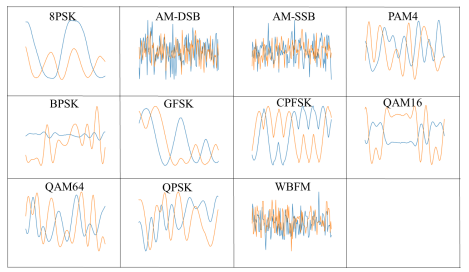
\includegraphics[width=0.9\textwidth]{figure/image5.png}
    \caption{数据集各调制类型波形图}
    \label{fig:dataset_waveform}
\end{figure}

\subsection{数据集可视化}
首先加载数据再对数据进行探索,在对数据集进行探索时,首先列出了不同信噪比(SNR)和调制类型的值,通过对数据集的进一步探索,计算了总的样本数量,并展示了每种调制类型的样本数目。

为了更好地理解数据集中的无线电信号特性,本文通过时域信号展示和IQ 星座图对信号进行了可视化。

时域信号展示能够直观地反映信号的振幅随时间的变化,有助于观察信号的周期性、幅度和噪声水平。通过绘制不同调制类型在特定信噪比下的I和Q通道时域波形,我们可以初步判断信号的特征。

\begin{figure}[H]
    \centering
    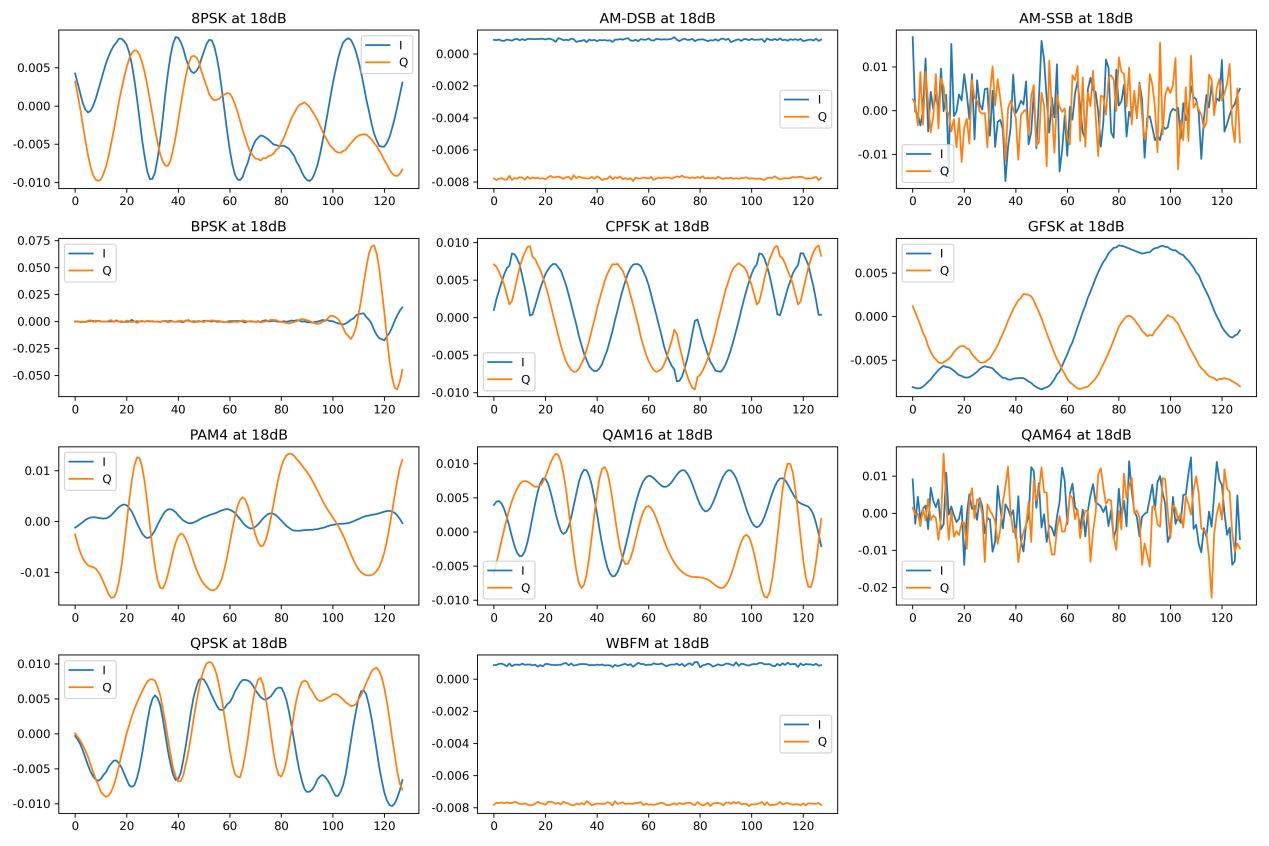
\includegraphics[width=0.9\textwidth]{figure/image6.png}
    \caption{时域信号示意图}
    \label{fig:time_domain_signal}
\end{figure}

IQ 星座图则将I和Q分量作为直角坐标系中的横轴和纵轴,每个采样点对应一个点。这使得我们可以清晰地观察到不同调制方式的符号映射方式。

\begin{figure}[H]
    \centering
    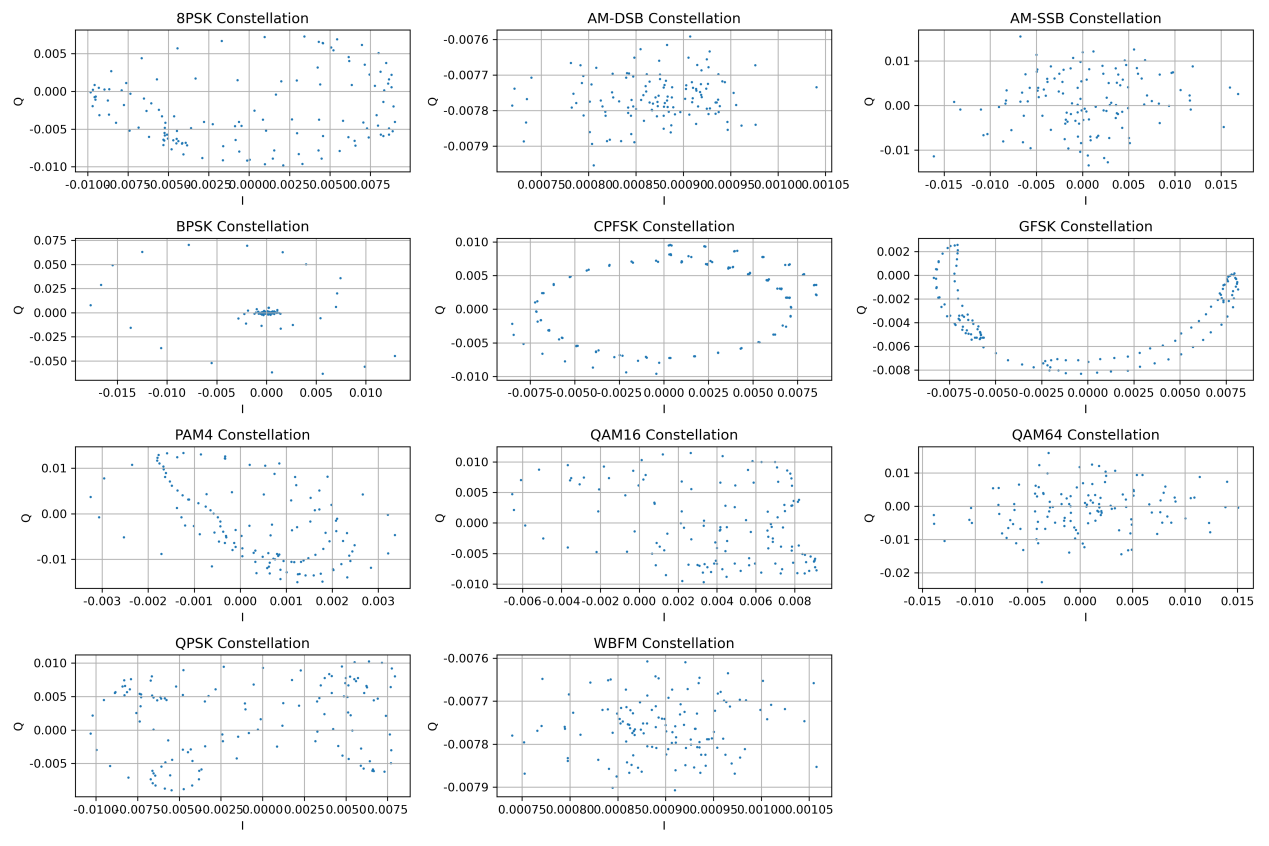
\includegraphics[width=0.9\textwidth]{figure/image7.png}
    \caption{IQ星座图}
    \label{fig:iq_constellation}
\end{figure}

\subsection{数据预处理}

\subsubsection{高斯过程回归去噪}
为了增强模型在低信噪比条件下的分类性能,本研究引入了基于高斯过程回归(GPR)的自适应去噪方法。在实际无线通信系统中,接收信号通常受到加性高斯白噪声(AWGN)的干扰,其中 $v[n]\sim\mathcal{CN}(0,\sigma_{n}^{2})$ 表示方差为$\sigma_{n}^{2}$的复高斯白噪声。GPR作为一种非参数贝叶斯方法,能够有效建模信号的潜在结构并抑制这种加性高斯白噪声的干扰。GPR去噪的关键在于对噪声水平的准确估计,这通过GPR模型中的参数(即每分量噪声方差)来实现。对于接收到的含噪信号 $r[n]=r_{I}[n]+jr_{Q}[n]$ 其平均功率定义为 $P_{r}=\mathbb{E}[|r[n]|^{2}]$。在实际中,若有M个离散时间样本,该平均功率通过对这些接收信号样本$r[k]$ ($k=0,...,M-1$)的瞬时功率 $(r_{I}[k]^{2}+r_{Q}[k]^{2})$ 求和并取平均来估计:
\begin{equation}
    P_{r}=\frac{1}{M}\sum_{k=0}^{M-1}(r_{I}[k]^{2}+r_{Q}[k]^{2})
    \label{eq:Pr}
\end{equation}
假设原始无噪信号$s[n]$的功率为 $P_{s}=\mathbb{E}[|s[n]|^{2}]$,噪声$w[n]$的功率为 $P_{w}=\mathbb{E}[|w[n]|^{2}]$。若信号与噪声不相关,则接收信号的总平均功率为:
\begin{equation}
    P_{r}=P_{s}+P_{w}
    \label{eq:Pr_sum}
\end{equation}
信噪比(SNR)定义为原始信号功率与噪声功率之比。其线性值为 $SNR_{linear}=P_{s}/P_{w}$,对应的分贝(dB)值为 $SNR_{dB}=10\log_{10}(SNR_{linear})$。利用此定义,可得 $P_{s}=SNR_{linear}\cdot P_{w}$。将其代入总功率关系式,有 $P_{r}=SNR_{linear}\cdot P_{w}+P_{w}=P_{w}(SNR_{linear}+1)$。因此,噪声功率可以根据实测信号功率$P_{r}$和给定的SNR计算得出:
\begin{equation}
    P_{w}=\frac{P_{r}}{SNR_{linear}+1}=\frac{P_{r}}{10^{SNR_{dB}/10}+1}
    \label{eq:Pw}
\end{equation}
对于复高斯白噪声 $w[n]=w_{I}[n]+jw_{Q}[n]$,其中同相分量 $w_{I}[n]$和正交分量 $w_{Q}[n]$相互独立且均服从零均值方差为 $\sigma_{n}^{2}$ 的正态分布,即 $w_{I}[n],w_{Q}[n]\sim\mathcal{N}(0,\sigma_{n}^{2})$。其噪声总功率定义为:
\begin{equation}
    P_{r}=\frac{1}{M}\sum_{k=0}^{M-1}(r_{I}[k]^{2}+r_{Q}[k]^{2})
    \label{eq:Pr_again}
\end{equation}
由此可得单个分量的噪声方差:
\begin{equation}
    \sigma_{n}^{2}=\frac{P_{w}}{2}
    \label{eq:sigma_n_squared}
\end{equation}
噪声标准差为:
\begin{equation}
    \sigma_{n}=\sqrt{\frac{P_{w}}{2}}
    \label{eq:sigma_n}
\end{equation}
结合式中 $P_{w}=\frac{P_{r}}{10^{SNR_{dB}/10}+1},$ 可进一步得到:
\begin{equation}
    \sigma_{n}=\sqrt{\frac{P_{r}}{2(10^{\frac{SNR_{dB}}{10}+1)}}}
    \label{eq:sigma_n_final}
\end{equation}
此即为GPR模型中设置的噪声水平参数。模型中采用径向基函数(RBF)、Matern 和 Rational Quadratic 等核函数分别描述信号的平滑特性。在去噪过程中,将离散时间索引 $X=[0,1,...,127]$ 作为输入,自身的同相或正交分量作为观测目标,通过噪声参数 $\alpha=\sigma_{n}^{2}$ 加入到协方差矩阵中实现噪声抑制。

为了适应不同 SNR条件下信号的平滑需求,本研究设计了基于SNR的长度尺度自适应策略。在高斯过程回归中,长度尺度参数L控制着核函数的相关性范围,直接影响去噪效果的强度。对于RBF核函数,其表达式为:
\begin{equation}
    k(x_{i},x_{j})=\sigma_{f}^{2}\exp\left(-\frac{(x_{i}-x_{j})^{2}}{2L^{2}}\right)
    \label{eq:rbf_kernel}
\end{equation}
其中$\sigma_{f}^{2}$为信号方差,L为长度尺度参数。较大的L值意味着相距较远的数据点仍具有较强的相关性,从而产生更强的平滑效果;而较小的L值则使得平滑效果更加局部化,能够保留更多的信号细节。

在低SNR条件下,噪声幅度相对较大,此时若采用过大的长度尺度L,会导致以下问题:
\begin{enumerate}
    \item 信号特征过度平滑:当L值过大时,GPR会将距离较远的信号样本视为强相关,导致真实信号的快速变化(如调制信号的幅度和相位跳变)被误认为噪声而被平滑掉。这种过度平滑会使得不同调制方式的特征差异变得模糊。
    \item 时域细节丢失:数字调制信号包含重要的时域特征,如符号跳变点、瞬时频率变化等。过大的L会使这些细节特征被平滑消除,降低后续分类网络提取有效特征的能力。
    \item 相位信息损失:对于相位调制信号(如PSK、QAM),相位的快速变化是关键识别特征。过度平滑会导致相位信息的损失,严重影响分类准确率。基于上述分析,本研究提出自适应长度尺度策略:设基础长度尺度为$L_{0}$。当SNR $\ge$ 0dB时取$L = L_{0}$:当SNR $<$ 0dB时,按以下方式进行动态调整:
\end{enumerate}
\begin{equation}
    L=\max(L_{\min},L_{0}(1+SNR/20))
    \label{eq:adaptive_L}
\end{equation}
其中$L_{\min}$是预设的最小尺度。该策略的核心思想是:随着SNR的降低,逐渐减小长度尺度L,从而减弱平滑效果,在去除噪声的同时最大限度地保留信号的有效信息。

具体而言,当SNR=-20dB时,长度尺度调整为 $L=\max(L_{\min},L_{0}\times0)=L_{\min},$ 此时平滑效果最弱,优先保留信号细节;当SNR逐渐提高时,长度尺度相应增大,平滑效果增强。这种自适应机制在高SNR场景下保证充分的去噪效果,在低 SNR 场景下则通过减弱平滑强度来保留更多有用的信号特征,实现了去噪性能与信号保真度之间的最优平衡。

去噪后的同相和正交分量重构为复数信号,作为后续神经网络训练的输入数据。

\subsubsection{旋转数据增强}
考虑到数字调制信号星座图的旋转对称性,本研究针对具有旋转对称性的调制类型(如PSK、QAM)采用基于复平面的旋转数据增强策略,以增强模型的泛化能力和对相位偏移的鲁棒性。对于非对称调制类型(如AM-SSB), 不应用旋转增强,以避免性能下降。对于复数信号$s[n]=s_{I}[n]+js_{Q}[n]$,旋转通过以下数学操作实现:将复数信号表示为向量 $[s_{I}[n],s_{Q}[n]]^{T}$,通过与旋转矩阵$R(\theta)$ 相乘实现旋转:
\begin{equation}
    \begin{bmatrix}
        S_{I}^{\prime}[n]\\
        S_{Q}^{\prime}[n]
    \end{bmatrix}
    =
    \begin{bmatrix}
        \cos\theta & -\sin\theta\\
        \sin\theta & \cos\theta
    \end{bmatrix}
    \begin{bmatrix}
        S_{I}[n]\\
        s_{Q}[n]
    \end{bmatrix}
    \label{eq:rotation_matrix}
\end{equation}
其中, $s_{I}^{\prime}[n]$和$s_{Q}^{\prime}[n]$是旋转后的同相和正交分量,$\theta$是旋转角度。在实现中,数据增强算法以输入数据张量 $X_{data}$(形状为 $(N,2,L)$,其中N是样本数,L是序列长度)和旋转角度 $\theta_{rad}$ 为参数。首先分离原始I和Q分量,应用旋转变换矩阵,然后重新组合成增强数据样本。基于调制类型的对称性,主要使用 $90^{\circ}(\pi/2)$、$180^{\circ}(\pi)$ 和 $270^{\circ}(3\pi/2)$ 的旋转,仅对具有旋转对称性的调制类型(如PSK、QAM)应用此策略。此方法有效将训练数据集扩展四倍,同时保留调制特征。通过学习旋转不变的特征表示,模型能够更好地处理由于载波相位偏移、多普勒效应等引起的信号旋转。

\newpage
\section{基于混合复值残差网络的信号分类模型}
本文首先对各类基础模型进行了对比研究,发现复值神经网络和ResNet 模型在RadioML 2016.10a数据集上分类性能较为优秀,再通过复值残差块设计、渐进式复-实转换和注意力增强机制结合了复值神经网络收敛速度快和 ResNet 预测精度高的优势,建立了混合复值残差网络模型,在数据集上达到了最佳性能。

\subsection{复值神经网络}
\subsubsection{引言}
复值神经网络(Complex-Valued Neural Network Modules, CVNN)是一个对基础神经网络模块进行复值化的GitHub开源项目。与传统实数神经网络(Real-Valued Neural Network, RVNN)不同,CVNN的参数和激活值均为复数,可以直接处理无线电信号中的I/Q分量。此外,其在深度状态空间模型(deep SSM)和大预言模型(LLMS)中也有广泛的应用。

\subsubsection{模型架构}
\begin{enumerate}
    \item 输入预处理层 \\
    输入信号初始形状为(2,128),表示128个时间步长的I/O序号,其中实部虚部分离存储,通过维度重排将输入信号转换为(128,2)的张量,实现时序-复数域对齐。
    \item 特征提取主干网络 \\
    特征提取主干网络由三级级联复数卷积模块构成,它的核心特征提取单元由三个深度复数卷积块构成,包含复数卷积、批归一化、激活函数和池化操作,形成层级化特征抽象网络,具体卷积模块构造如下:
    \begin{itemize}
        \item 复数卷积层(ComplexConv1D) \\
        复数卷积层包含三级滤波器组,第一级为64个5$\times$5复数滤波器,捕获粗粒度时空特征,第二级为128个5$\times$5复数滤波器,提取中级语义特征,第三级为256个3$\times$3复数滤波器,进行精细特征编码。通过公式(3):
        \begin{equation}
            (a+jb)\otimes(c+jd)=(ac-bd)+j(ad+bc)
            \label{eq:complex_conv}
        \end{equation}
        实现实部权重矩阵$W_{real}$和虛部权重矩阵$W_{imag}$,并行计算四个卷积通道$(conv_{rr},conv_{ri},conv_{ir},conv_{ii})$ 最终合成复数特称图。
        \item 复数批归一化层(ComplexBatchNormalization) \\
        复数批归一化层包含协方差矩阵计算模块,白化变换模块和自适应缩放模块。
        协方差矩阵计算模块通过公式(X)统计三个协方差分量:
        \begin{equation}
            V_{rr} = E[x_{real}], V_{ii} = E[x_{imag}], V_{ri}=E[x_{real}x_{imag}]
            \label{eq:covariance}
        \end{equation}
        白化变换模块通过Cholesky 分解实现数据去相关,保留复数域能量:
        \begin{equation}
            \hat{x}=\Lambda^{-\frac{1}{2}}U^{H}(x-\mu)
            \label{eq:whitening_transform}
        \end{equation}
        其中U为协方差矩阵的特征向量矩阵,$\Lambda$为特征值对角矩阵。
        自适应缩放模块通过使用可学习的缩放参数$\gamma_{rr}$, $\gamma_{ri}$ 进行幅度校正,保持复数域的自由度。
        \item 复数激活层(ComplexActivation) \\
        复数激活层支持 modReLU/Cardioid/CReLU等7种激活函数,通过 activation\_type 参数进行动态配置调整,以modReLU为例,其数学表达式为:
        \begin{equation}
            \sigma(z)=\text{ReLU}(|z|+b)\cdot\frac{z}{|z|}
            \label{eq:modrelu}
        \end{equation}
        modReLU函数通过阈值化幅度同时保留相位信息,相比实数ReLU在复数域具有更好的特征表达能力。
        \item 复数池化层(ComplexPooling1D) \\
        复数池化层通过引入时域下采样方法,通过步长采样实现特征图尺寸减半(128$\rightarrow$64$\rightarrow$32),有效扩大感受野,此外采用了简单采样策略(非传统最大池化),避免了相位跳跃导致的特征失真。
    \end{itemize}
    \item 全局特征聚合器 \\
    全局特征聚合器通过全局平均池化实现时空维度的深度压缩。该层接收形状为(32,256)的复数特征图,对每个特征通道计算时间维度上的均值:
    \begin{equation}
        \hat{x}_{c}=\frac{1}{T}\sum_{t=1}^{T}x_{c,t}
        \label{eq:global_avg_pooling}
    \end{equation}
    其中T为时间步数,c为特征通道索引。
    \item 分类决策系统 \\
    分类决策系统构建了双通道复数推理引擎。首层配置512个复数单元,通过复数矩阵乘法实现特征空间扩展,其运算过程遵循以下公式:
    \begin{equation}
        y_{real}=x_{real}W_{real}-x_{imag}W_{imag} \\
        y_{imag}=x_{real}W_{imag}+x_{imag}W_{real}
        \label{eq:complex_linear}
    \end{equation}
    其中 $W_{real},W_{imag}\in\mathbb{R}^{256\times512}$ 为分离的实部/虛部权重矩阵。激活函数采用 modReLU函数,在保留相位特征的同时引入非线性表达能力,之后配合0.5比例的Dropout 层实现动态正则化。次层256个复数单元进一步融合高层特征,使用Cardioid 激活函数进行相位选择性抑制:
    \begin{equation}
        \text{Cardioid}(z)=0.5\cdot(1+\cos\theta)\cdot z
        \label{eq:cardioid}
    \end{equation}
    选择性抑制后通过0.3比例的Dropout 提升泛化性能。最终通过幅度映射层进行模长计算:
    \begin{equation}
        |z|=\sqrt{\text{Re}(z)^{2}+\text{Im}(z)^{2}}
        \label{eq:magnitude}
    \end{equation}
    \item 输出层 \\
    输出层采用全连接分类器与Softmax函数的组合。分类器通过权重矩阵$W\in\mathbb{R}^{256\times C}$ 实现特征空间到类别空间的线性映射,输出节点数严格对应任务类别数。Softmax 函数对原始得分进行概率归一化:
    \begin{equation}
        p_{i}=\frac{e^{z_{i}}}{\sum_{k=1}^{c}e^{z_{k}}}
        \label{eq:softmax}
    \end{equation}
    归一化后生成有效的类别概率分布。配合交叉熵损失函数:
    \begin{equation}
        L=-\sum_{i=1}^{c}y_{i}\log(p_{i})
        \label{eq:cross_entropy}
    \end{equation}
    构建端到端优化目标,使模型在RML2016.10a基准数据集上达到较高的调制识别准确率。
\end{enumerate}

\subsection{ResNet 模型}
\subsubsection{引言}
ResNet (Residual Network)的核心创新是通过残差学习框架引入跨层跳跃连接,允许梯度直接绕过非线性层传播,有效解决了深层网络训练中的梯度消失与性能退化问题。典型残差块通过两个卷积层堆叠后与输入进行逐元素相加 $(H(x)=F(x)+x)$,使网络可轻松训练至百层深度。

\subsubsection{模型架构}
\begin{enumerate}
    \item 输入预处理层 \\
    通过维度置换操作将输入张量 $X\in \mathbb{R}^{B\times C\times T}$ 转换为 $X^{\prime}\in\mathbb{R}^{B\times T\times C}$ 其中B为批次大小,$C=2$ 为I/Q 通道数,$T=128$ 为时序长度。
    \item 初始特征提取模块 \\
    采用大核卷积捕获时频域联合特征:
    \begin{equation}
        Y=\sigma(\text{BN}(W_{1}*X^{\prime}+b_{1}))
        \label{eq:initial_feature}
    \end{equation}
    其中 $W_{1}\in\mathbb{R}^{7\times C\times64}$ 为7$\times$1卷积核,*表示一维卷积操作, $\sigma(\cdot)=\max(0,\cdot)$ 为ReLU激活, $\text{BN}(\cdot)$ 为批归一化。
    \item 残差学习模块 \\
    残差学习模块包含三级残差块,每级由两个卷积层构成,分别为恒等映射:
    \begin{equation}
        F_{1}=W_{2}^{(3)}*\sigma(\text{BN}(W_{2}^{(3)}*P+b_{2}^{(1)})+b_{2}^{(2)})
        \label{eq:residual_identity1}
    \end{equation}
    \begin{equation}
        R_{1}=\sigma(F_{1}+P)
        \label{eq:residual_identity2}
    \end{equation}
    带下采样:
    \begin{equation}
        S_{2}=\text{Conv}(R_{1},\text{stride}=2)
        \label{eq:downsample1}
    \end{equation}
    \begin{equation}
        F_{2}=W_{3}^{(3)}*\sigma(\text{BN}(W_{3}^{(3)}*S_{2}+b_{3}^{(1)})+b_{3}^{(2)})
        \label{eq:residual_downsample1}
    \end{equation}
    \begin{equation}
        R_{2}=\sigma(F_{2}+S_{2})
        \label{eq:residual_downsample2}
    \end{equation}
    特征深化:
    \begin{equation}
        S_{3}=\text{Conv}(R_{2},\text{stride}=2)
        \label{eq:downsample2}
    \end{equation}
    \begin{equation}
        F_{3}=W_{4}^{(3)}*\sigma(\text{BN}(W_{4}^{(3)}*S_{3}+b_{4}^{(1)})+b_{4}^{(2)})
        \label{eq:residual_deepen1}
    \end{equation}
    \begin{equation}
        R_{3}=\sigma(F_{3}+S_{3})
        \label{eq:residual_deepen2}
    \end{equation}
    \item 分类决策模块 \\
    分类决策模块通过全局平均池化压缩时序维度,之后连接全连接层进行特征融合。
\end{enumerate}
ResNet 模型通过残差连接缓解梯度消失,结合批归一化和ReLU 激活实现稳定训练,通过特别设计的大核卷积与多级下采样结构使得模型适用于无线电信号分类任务。

\subsection{混合复值残差网络模型}
\subsubsection{引言}
随着无线通信技术的快速发展,复杂电磁环境下的信号分类任务(如调制识别、频谱感知)对模型的鲁棒性和特征表达能力提出了更高要求。传统的深度学习方法通常将复数I/Q 信号拆分为实部和虚部分别处理,导致相位信息的丢失和模型收敛速度的下降。针对这一问题,本文提出了一种混合复值残差网络模型(Hybrid Complex-ResNet Model, HCRM),通过将复值神经网络(ComplexNN)的快速收敛特性与残差网络(ResNet)的深度学习能力相结合,实现了对I/Q信号的端到端复数域处理。
该模型的核心创新包括:
\begin{enumerate}
    \item 复值残差块设计:通过复数卷积、批归一化和跳跃连接,在保留信号相位信息的同时缓解梯度消失问题;
    \item 渐进式复-实转换:仅在分类层前将复数特征转换为实数模值,避免早期信息损失;
    \item 注意力增强机制:在深层残差块中引入复数注意力模块,提升对多尺度特征的提取能力。
\end{enumerate}
实验结果表明,该模型在无线电信号分类任务中显著优于传统实值网络,尤其在低信噪比环境下展现出更强的泛化性能。该模型为复值信号处理提供了新的深度学习范式,为智能无线电系统中的实时信号分析提供了理论支撑和技术方案。

\subsubsection{网络架构设计}
\begin{enumerate}
    \item 输入处理与初始特征提取 \\
    模型接收形状为(2,128)的I/Q信号输入,首先通过Permute 层重组维度为(128,2)以适配复数卷积操作。初始特征提取阶段采用7$\times$1复数卷积(64 filters)进行频谱特征映射,配合复数批归一化(ComplexBatchNormalization)和复数 Leaky ReLU激活函数实现快速收敛。随后通过2-stride 复数最大池化(ComplexPooling1D)进行下采样,生成(64,64)尺寸的特征图。
    \item 复数残差学习骨干网络 \\
    模型核心由两级复数残差块构成深度特征提取网络,分别为基础复数残差块和高级复数残差块
    \begin{itemize}
        \item 基础复数残差块:采用双3$\times$1复数卷积结构,配合捷径连接实现恒等映射。当输入输出维度不匹配时,通过1$\times$1复数卷积进行维度对齐,残差连接采用复数加法 $\hat{x}_{l+1}=F(x_{l})+x_{l},$ 其中F表示残差映射函数。
        \item 高级复数残差块:引入三阶段处理流程(3$\times$1$\rightarrow$3$\times$1$\rightarrow$1$\times$1卷积)和可选注意力机制。注意力分支通过1$\times$1复数卷积生成权重W,与输入特征进行复数乘法:
        \begin{equation}
            y=(x_{r}W_{r}-x_{i}W_{i}) + j(x_{r}W_{i} + x_{i}W_{r})
            \label{eq:complex_attention}
        \end{equation}
    \end{itemize}
    \item 渐进式域转换机制 \\
    渐进式域转换机制通过混合过渡块(HybridTransitionBlock,HTB)实现特征空间的平滑过渡,HTB包含以下两个主要特征:
    \begin{itemize}
        \item 动态滤波器分配:根据预设的transition\_ratio 参数,将滤波器划分为复数分支和实数分支。例如当ratio 0.7时,256个滤波器中179个用于复数处理,77个用于实数处理。
        \item 双路径处理:
        \begin{itemize}
            \item 复数路径:3$\times$1复数卷积$\rightarrow$批归一化$\rightarrow$Leaky ReLU 激活$\rightarrow$幅值转换(ComplexMagnitude)
            \item 实数路径:直接提取输入幅值$\rightarrow$3$\times$1实数卷积$\rightarrow$批归一化$\rightarrow$ReLU激活函数。
        \end{itemize}
    \end{itemize}
    \item 传统 ResNet 增强模块 \\
    在特征图转换为实数域后,模型采用经典 Bottleneck 结构进行深度特征提炼,Bottleneck 结构通过以下三步进行处理:
    \begin{enumerate}
        \item 残差单元:由1$\times$1降维卷积$\rightarrow$3$\times$3 卷积$\rightarrow$1$\times$1升维卷积构成,使用批归一化和ReLU激活函数。
        \item 下采样处理:通过2-stride卷积实现空间维度压缩,捷径连接采用1$\times$1卷积进行维度匹配。
        \item 层次化特征:通过三级残差块(512 filters)提取多尺度上下文信息,最终通过全局平均池化(GlobalAveragePooling1D)生成特征向量。
    \end{enumerate}
    \item 分类决策系统模块 \\
    分类决策系统模块包含深度特征精炼、残差增强和最终分类三步。
    \begin{enumerate}
        \item 深度特征精炼 \\
        深度特征精炼首先使用两个全连接层(分别为1024个单元和512个单元)对全局特征向量进行深度精炼,再通过Dropout层(分别设置0.5和0.3的丢弃率)防止过拟合,从而既能提取高级语义特征,也提高了模型的泛化能力。
        \item 残差增强 \\
        模型通过跳跃连接将全局池化前的特征与倒数第二层全连接层的输出相加,增强信息流动和梯度传播。
        \item 最终分类 \\
        将256维 ReLU全连接层后接Softmax输出层,生成类别概率分布:
        \begin{equation}
            P(y=i|x)=\frac{e^{w_{i}^{T}x+b_{i}}}{\sum_{j=1}^{K}e^{w_{j}^{T}x+b_{j}}}
            \label{eq:softmax_final}
        \end{equation}
        其中,K为类别数,$w_{i}$和$b_{i}$分别为第i类的权重向量和偏置项。
    \end{enumerate}
\end{enumerate}

\begin{figure}[H]
    \centering
    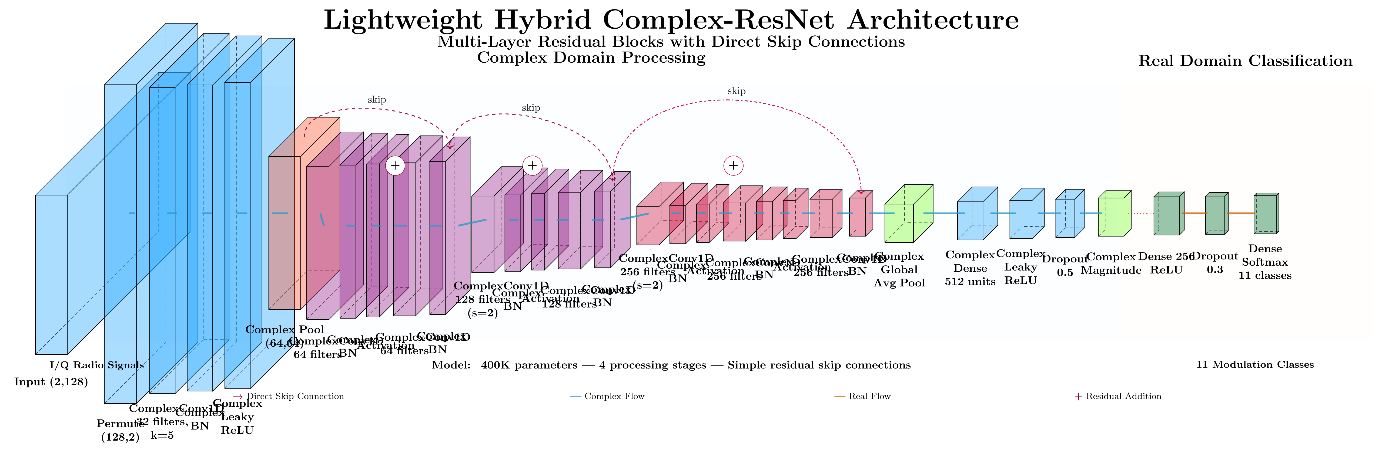
\includegraphics[width=0.9\textwidth]{figure/image8.png}
    \caption{混合复值残差网络模型架构图}
    \label{fig:hybrid_architecture}
\end{figure}

\subsubsection{模型训练与参数回调}
\begin{enumerate}
    \item 训练策略 \\
    训练策略包含动态学习率、正则化体系和损失函数三个模块。
    动态学习率采用指数衰减策略,初始学习率 $\eta_{0}=0.002$,每1000步以衰减率 $\gamma=0.95$ 进行衰减:
    \begin{equation}
        \eta_{t}=\eta_{0}\cdot\gamma^{[\frac{t}{1000}]}
        \label{eq:learning_rate_decay}
    \end{equation}
    模型在复数路径中使用L2正则化(权重衰减 $\lambda=10^{-4})$,实数路径采用 Dropout 和批归一化进行协同正则化。
    损失函数通过加权分类交叉熵损失,通过类权重平衡技术缓解类别不平衡问题:
    \begin{equation}
        \mathcal{L}=-\sum_{i=1}^{k}w_{i}y_{i}\log(P(y_{i}|x))
        \label{eq:weighted_cross_entropy}
    \end{equation}
    \item 激活函数的选择 \\
    在模型中,好的激活函数能引入非线性,让模型能学习复杂模式,提升表达能力;可加速训练收敛,使模型更快达到较好状态;还有助于提高模型准确性,更好地拟合数据;同时还能增强模型鲁棒性,缓解梯度消失等问题,使模型对输入变化不那么敏感。

    本文比较在复数域内较常用的六种激活函数,最终选择了最适合I/Q数据集的modReLU函数。

    \begin{table}[H]
        \centering
        \caption{激活函数性能表}
        \begin{tabular}{|l|c|c|c|c|}
            \hline
            \textbf{激活函数} & \textbf{相位保持} & \textbf{计算效率} & \textbf{训练稳定性} & \textbf{信号处理适用性} \\
            \hline
            complex\_relu & X & $\star\star\star$ & $\star\star$ & $\star$ \\
            \hline
            mod\_relu & $\checkmark$ & $\star\star$ & $\star\star\star$ & $\star\star\star\star$ \\
            \hline
            zrelu & $\checkmark$ & $\star\star\star$ & $\star\star$ & $\star\star\star$ \\
            \hline
            cardioid & $\checkmark$ & $\star\star$ & $\star\star\star$ & $\star\star\star$ \\
            \hline
            complex\_tanh & X & $\star\star$ & $\star\star$ & $\star\star$ \\
            \hline
            phase\_amplitude & $\checkmark$ & $\star\star$ & $\star\star\star$ & $\star\star\star$ \\
            \hline
        \end{tabular}
        \label{tab:activation_functions}
    \end{table}

    \item 模型训练
    \begin{enumerate}
        \item 环境初始化 \\
        设置随机种子确保结果可复现,设置batch\_size为128,最大训练步长epoch为100,划分训练集、测试集、验证集的比例为0.72:0.2:0.08。
        \item 模型训练 \\
        模型采用渐进式训练策略: 首先训练基线模型,然后依次加入GPR去噪、旋转数据增强和混合架构,每个阶段独立训练并记录性能提升,最终训练包含所有改进的完整模型。
        将数据输入 HCRM 模型中进行训练后,模型会在每个epoch 结束后使用验证集(X\_val, y\_val)来评估性能,包括计算准确率和损失,同时也会保存训练集上的准确率和损失函数。
        \item 参数回调 \\
        本文将三个核心回调函数进行组合应用以优化模型训练过程,模型检查点函数会在每个时间步长结束后评估验证集表现,当发现当前验证准确率优于历史记录时,自动将模型权重进行保存;学习率衰减函数会在当连续2个epoch指标无提升时触发,按比例衰减学习率,并会在学习率小于等于$1e-6$时停止衰减;提前终止函数将在模型性能连续30个时间步长未提升时触发,自动选择最优权重终止模型进程。
    \end{enumerate}
\end{enumerate}
通过上述三个回调函数,有效防止了因过拟合导致的模型性能下降,训练过程中准确率和损失函数的过激震荡,以及无效训练迭代导致的性能浪费,其触发逻辑如下图:

\begin{figure}[H]
    \centering
    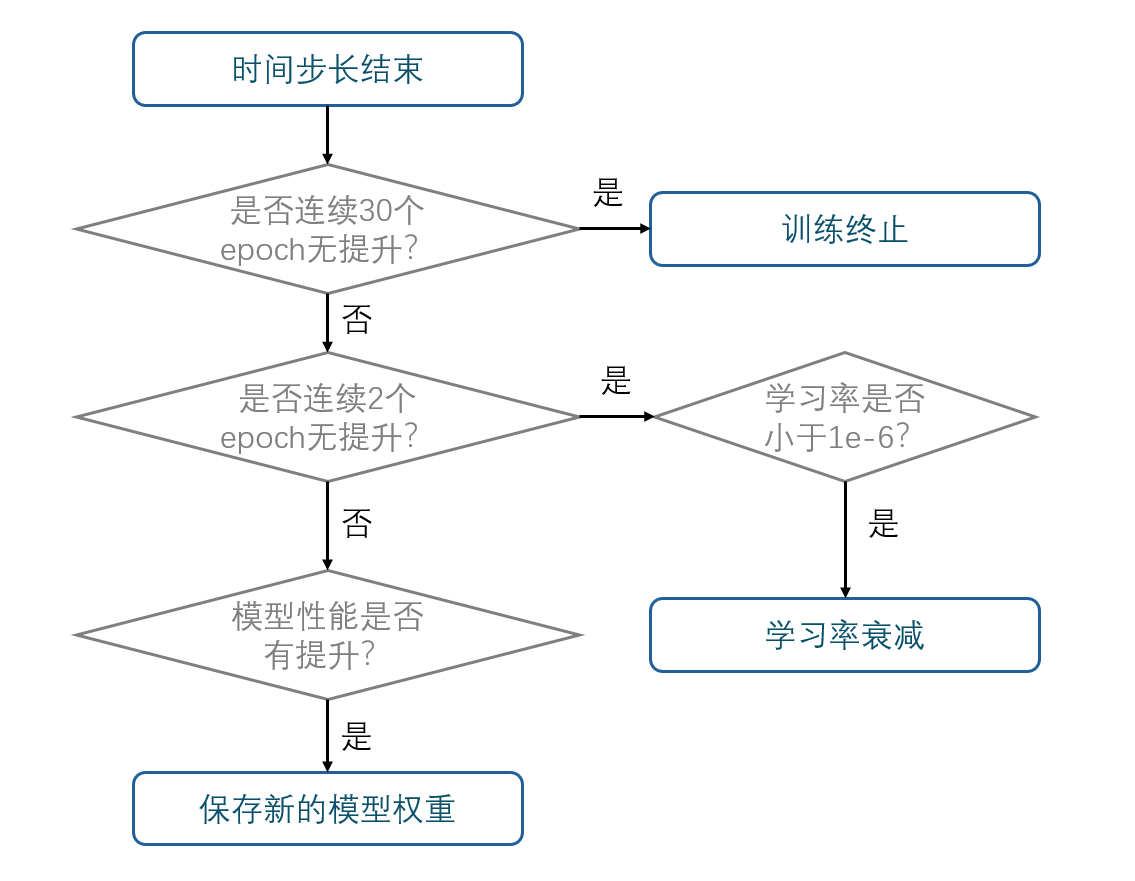
\includegraphics[width=0.7\textwidth]{figure/image9.png}
    \caption{参数回调逻辑流程图}
    \label{fig:callback_logic}
\end{figure}

模型训练完成后,得到epoch-accuracy\&loss曲线如下图:

\begin{figure}[H]
    \centering
    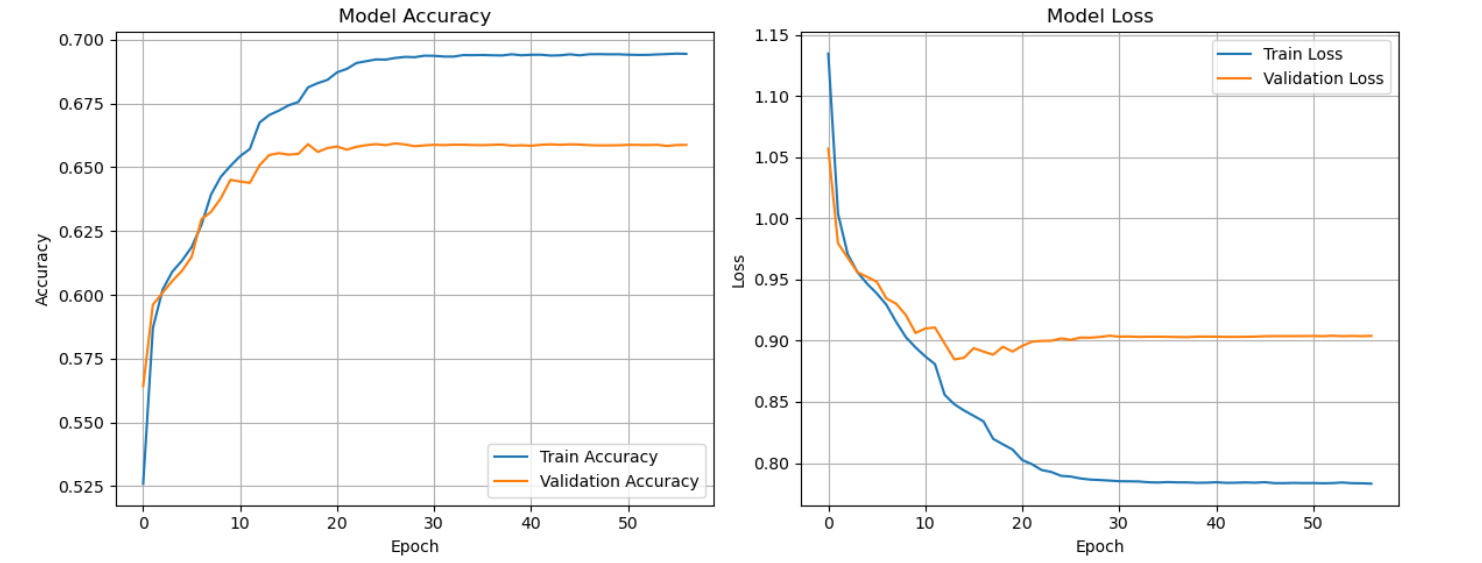
\includegraphics[width=0.9\textwidth]{figure/image10.png}
    \caption{epoch-accuracy\&loss 曲线}
    \label{fig:epoch_curve}
\end{figure}

可以看出,模型收敛速度快,仅在20个时间步长左右就收敛到了最优准确率,同时也没有出现明显的震荡现象,在验证集上的准确率表现优异。

\subsection{本章小结}
本章提出的混合复值残差网络模型(HCRM)针对复杂电磁环境下的信号分类任务提出了三项核心创新。通过复值残差块设计将复数卷积、批归一化与跳跃连接结合,在保留I/Q信号相位信息的同时缓解梯度消失问题,为复数域深度学习提供了新的结构范式。渐进式复-实转换机制通过混合过渡块实现特征域平滑过渡,利用动态滤波器分配策略在复数路径与实数路径间建立协同,既保留了相位敏感性又避免了早期信息损失。在深层残差块中引入复数注意力模块,结合传统ResNet的Bottleneck 结构,构建了多尺度特征提取与信息融合的双重增强机制,显著提升了模型对调制细节的感知能力。

在模型训练层面,HCRM采用了动态优化与多维度正则化策略。通过指数衰减学习率(初始值0.002,衰减率0.95)与L2正则化构建基础优化框架,结合双阶段 Dropout(0.5/0.3丢弃率)形成协同正则化体系。激活函数选择方面,经对比实验验证的modReLU 函数在相位保持特性与计算效率间取得平衡,尤其适配I/Q信号的非线性建模需求。训练过程中,模型检查点以验证集准确率为监控指标动态保存最优权重,学习率衰减机制在连续2个epoch无改进时触发,配合30个epoch耐心值的提前终止策略,构建了自动化训练保障体系。

\newpage
\section{实验结果与分析}

\subsection{整体分类性能}
设置学习率衰减容忍步长为2,终止迭代容忍步长为30,衰减因子为0.5。实验结果表明,HCRM 模型在RadioML 2016.10a数据集上的分类准确率优于其它模型,且显著优于传统模型。其在低信噪比的环境下仍然展现出对噪声较强的鲁棒性,模型的分类热力图如下:

\begin{figure}[H]
    \centering
    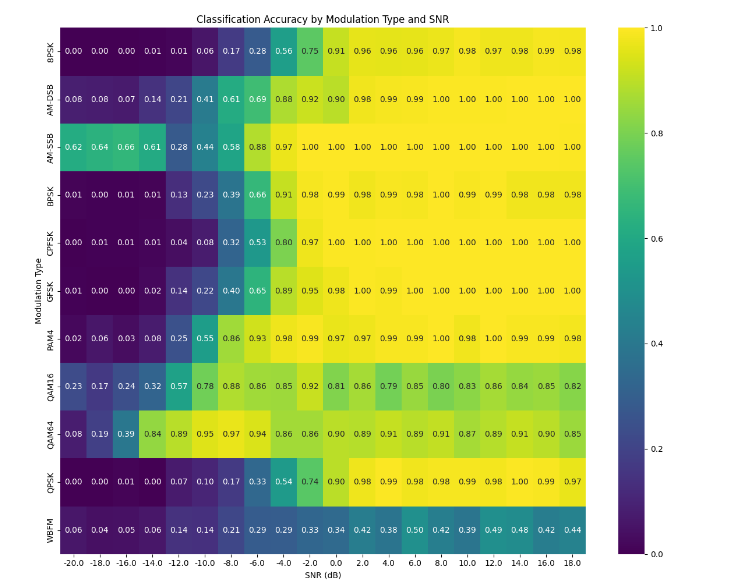
\includegraphics[width=0.9\textwidth]{figure/image11.png}
    \caption{HCRM 模型分类结果热力图}
    \label{fig:hcrm_heatmap}
\end{figure}

模型在不同信道下的分类性能如下表:

\begin{table}[H]
    \centering
    \caption{HCRM 模型分类性能表}
    \begin{tabular}{|l|c|c|c|c|}
        \hline
        \textbf{Channel} & \textbf{precision} & \textbf{recall} & \textbf{f1-score} & \textbf{support} \\
        \hline
        8PSK & 0.83 & 0.58 & 0.68 & 4000 \\
        AM-DSB & 0.50 & 0.71 & 0.59 & 4000 \\
        AM-SSB & 0.38 & 0.84 & 0.53 & 4000 \\
        BPSK & 0.77 & 0.65 & 0.70 & 4000 \\
        CPFSK & 0.87 & 0.64 & 0.74 & 4000 \\
        GFSK & 0.81 & 0.67 & 0.73 & 4000 \\
        PAM4 & 0.81 & 0.72 & 0.76 & 4000 \\
        QAM16 & 0.60 & 0.71 & 0.65 & 4000 \\
        QAM64 & 0.78 & 0.79 & 0.79 & 4000 \\
        QPSK & 0.82 & 0.58 & 0.68 & 4000 \\
        WBFM & 0.58 & 0.29 & 0.39 & 4000 \\
        \hline
        \textbf{accuracy} & \multicolumn{3}{|c|}{0.65} & \textbf{44000} \\
        \hline
        \textbf{macro avg} & 0.71 & 0.65 & 0.66 & 44000 \\
        \hline
        \textbf{weighted avg} & 0.71 & 0.65 & 0.66 & 44000 \\
        \hline
    \end{tabular}
    \label{tab:hcrm_performance}
\end{table}

从表格中可以看出HCRM模型在包含11种信道(8PSK、AM-DSB、AM-SSB、BPSK、CPFSK、GFSK、PAM4、QAM16、QAM64、QPSK、WBFM)的测试集上达到了0.6538的整体准确率,但存在较为明显的性能分化。

模型在QAM64和PAM4信道上表现优异,准确率、召回率、F1-score均处于领先水平,模型识别全面;在WBFM信道上性能不佳,召回率仅29\%,存在严重漏检问题;对于AM-SSB调制仅有0.38的准确率,存在大量误报,假阳性概率高;模型在QPSK 信道上精确率高,但是召回率低,识别较为保守;对于AM-DSB调制模型召回率高但是准确率低,存在过度预测现象,其余信道的表现较为均衡稳定,模型的混淆矩阵如下图:

\begin{figure}[H]
    \centering
    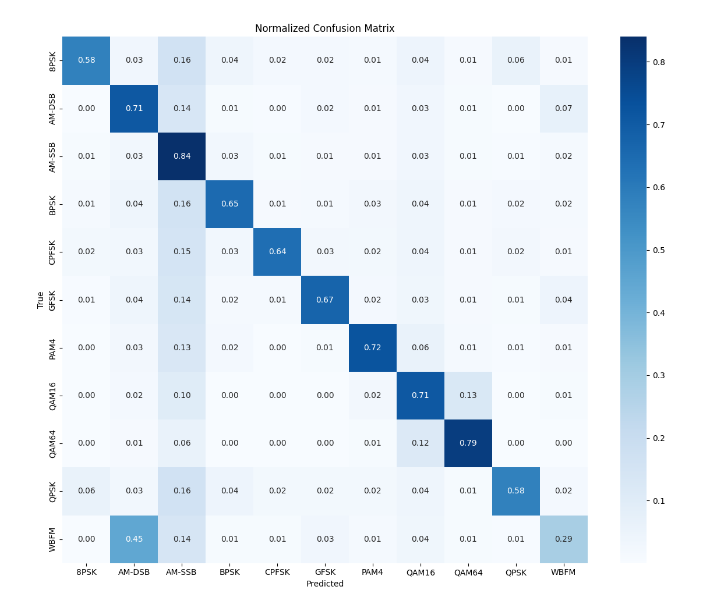
\includegraphics[width=0.9\textwidth]{figure/image12.png}
    \caption{HCRM 模型混淆矩阵}
    \label{fig:confusion_matrix}
\end{figure}

\subsection{信噪比敏感性分析}
RadioML 2016.10a数据集的SNR参数覆盖了-20dB至+18dB的宽幅度动态范围,步长为2dB。其中,低信噪比数据的噪声含量高,仅有少量的有效数据,可以用来检验模型在复杂电磁环境下的分类能力;而高信噪比则近似理想信道条件,可以用来验证模型对纯净信号的分类性能。数据集在每个信道的每个SNR上均有1000个样本。HCMR 模型的信噪比-准确率曲线如下图所示:

\begin{figure}[H]
    \centering
    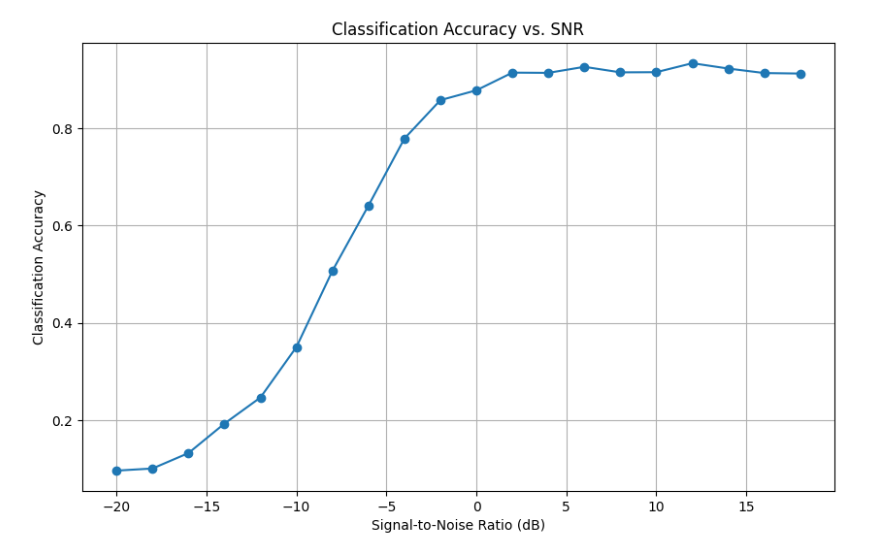
\includegraphics[width=0.9\textwidth]{figure/image13.png}
    \caption{信噪比-准确率曲线}
    \label{fig:snr_accuracy_curve}
\end{figure}

详细的准确率数据如下表:

\begin{table}[H]
    \centering
    \caption{SNR-accuracy 数据表}
    \begin{tabular}{|c|c|c|c|}
        \hline
        \textbf{SNR} & \textbf{accuracy} & \textbf{SNR} & \textbf{accuracy} \\
        \hline
        -20 & 0.0965 & -18 & 0.1008 \\
        \hline
        -16 & 0.1321 & -14 & 0.1931 \\
        \hline
        -12 & 0.2472 & -10 & 0.3505 \\
        \hline
        -8 & 0.5062 & -6 & 0.6405 \\
        \hline
        -4 & 0.7784 & -2 & 0.8573 \\
        \hline
        0 & 0.8780 & 2 & 0.9144 \\
        \hline
        4 & 0.9139 & 6 & 0.9263 \\
        \hline
        8 & 0.9154 & 10 & 0.9153 \\
        \hline
        12 & 0.9337 & 14 & 0.9227 \\
        \hline
        16 & 0.9135 & 18 & 0.9125 \\
        \hline
    \end{tabular}
    \label{tab:snr_accuracy_data}
\end{table}

信噪比-准确率曲线呈现先陡升后趋缓并伴随局部波动的特征:在-20dB至12dB区间准确率随SNR 提高显著增长,其中-20dB至0dB阶段准确率从9.65\%快速攀升至87.8\%,0dB至12dB期间增速放缓但仍提升至93.37\%的峰值;当SNR超过12dB后准确率后模型达到性能边界,出现小幅震荡。

\subsection{分类性能对比}
HCRM 模型与改进后的ComplexNN和ResNet的分类准确度对比图如下:

\begin{figure}[H]
    \centering
    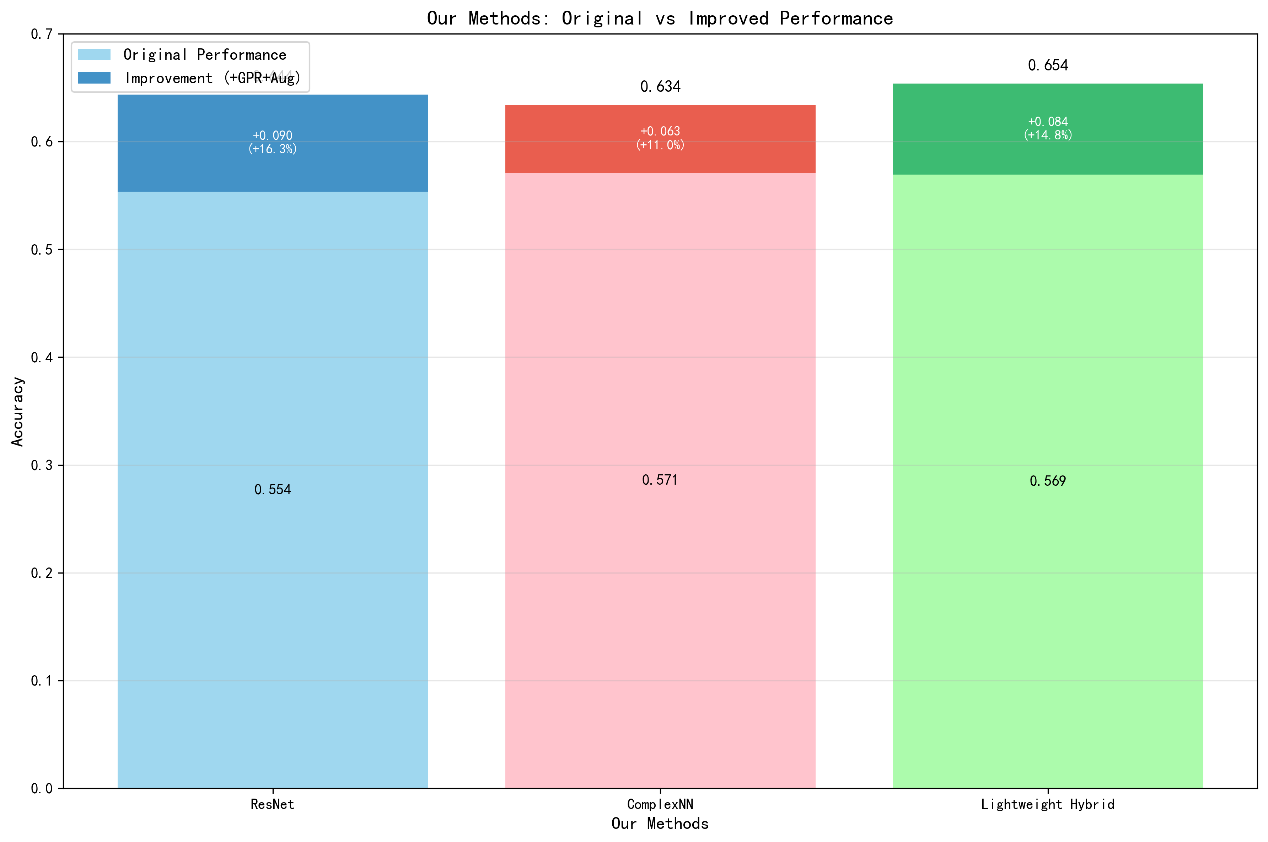
\includegraphics[width=0.9\textwidth]{figure/image14.png}
    \caption{改进模型性能对比图}
    \label{fig:improved_model_comparison}
\end{figure}

从图中可以看出高斯回归和旋转数据增强的数据预处理方法对于三种模型的分类性能均有普适的提升。在未应用数据预处理方法时,复值神经网络的分类准确率达到最高,为57.1\%,然而HCRM 模型更加适应预处理后的数据,最终达到了65.4\%的最高精度。

HCRM 模型与其它传统机器学习模型的性能对比图如下:

\begin{figure}[H]
    \centering
    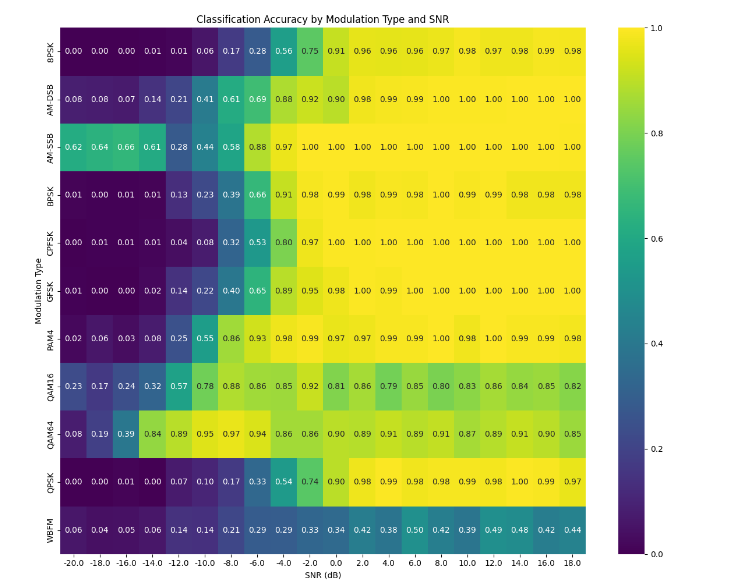
\includegraphics[width=0.45\textwidth]{figure/image11.png}
    \caption{HCRM 热力图}
    \label{fig:traditional_model_heatmap_hcrm}
\end{figure}
\begin{figure}[H]
    \centering
    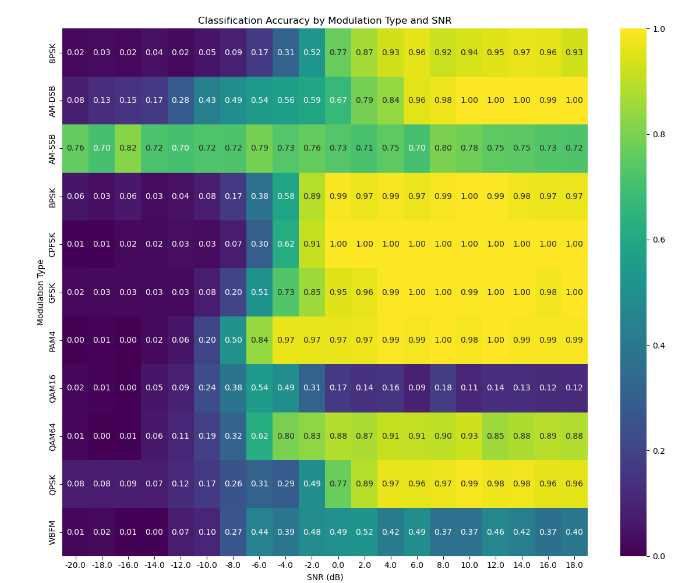
\includegraphics[width=0.45\textwidth]{figure/image15.png}
    \caption{CNN1d 热力图}
    \label{fig:traditional_model_heatmap_cnn1d}
\end{figure}
\begin{figure}[H]
    \centering
    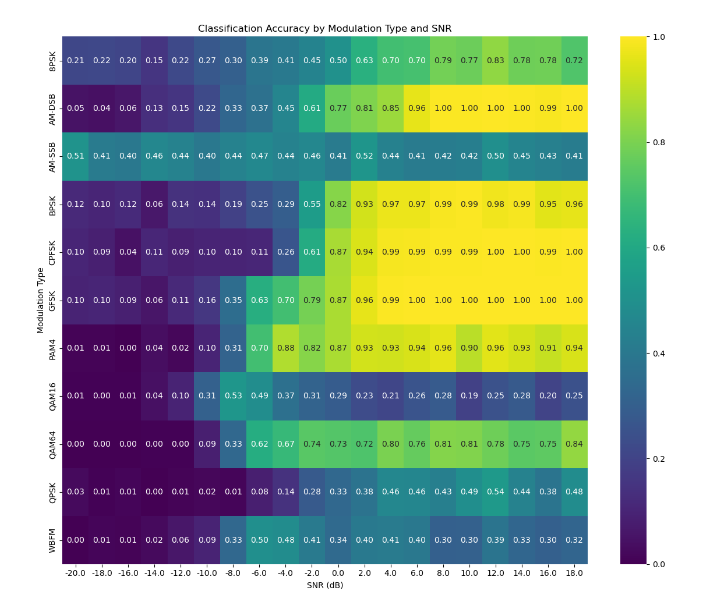
\includegraphics[width=0.45\textwidth]{figure/image16.png}
    \caption{CNN2d 热力图}
    \label{fig:traditional_model_heatmap_cnn2d}
\end{figure}
\begin{figure}[H]
    \centering
    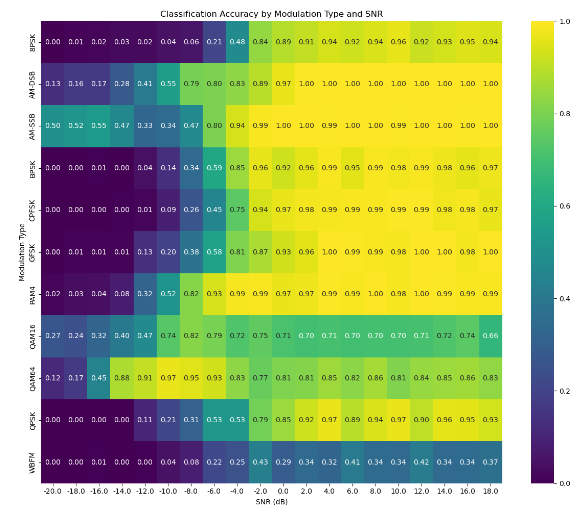
\includegraphics[width=0.45\textwidth]{figure/image17.png}
    \caption{CNN 热力图}
    \label{fig:traditional_model_heatmap_cnn}
\end{figure}
\begin{figure}[H]
    \centering
    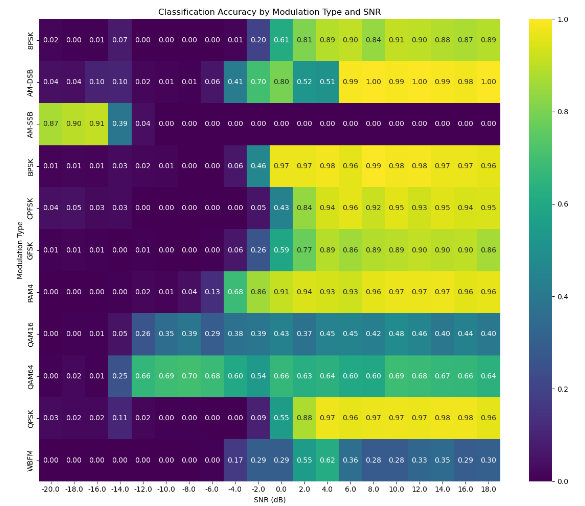
\includegraphics[width=0.45\textwidth]{figure/image18.png}
    \caption{Transformer 热力图}
    \label{fig:traditional_model_heatmap_transformer}
\end{figure}
\begin{figure}[H]
    \centering
    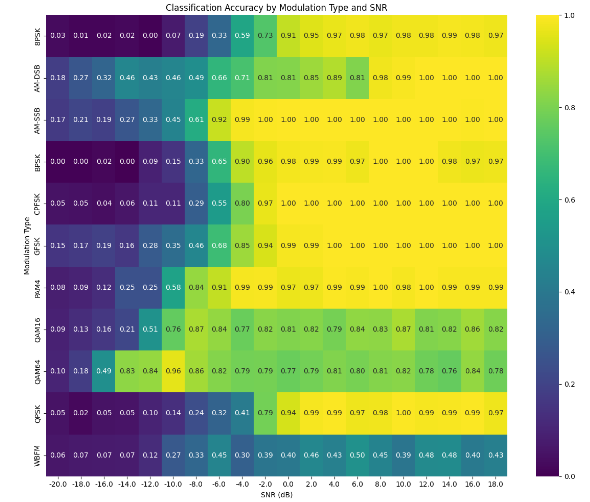
\includegraphics[width=0.45\textwidth]{figure/image19.png}
    \caption{ResNet 热力图}
    \label{fig:traditional_model_heatmap_resnet}
\end{figure}
从图中可以看出,得益于高斯回归和旋转数据增强的数据预处理手法,以及对复值神经网络和ResNet 模型的有机结合,HCMR 模型在 RadioML 2016.10a数据集上的表现远优于CNN1d, CNN, transformer 等传统机器学习模型。随后我们对上述图表进行整理,得到分类性能对比如下表:

\begin{table}[H]
    \centering
    \caption{分类性能对比表}
    \begin{tabular}{|l|c|}
        \hline
        \textbf{model} & \textbf{accuracy} \\
        \hline
        resnet+augment & 0.5934 \\
        \hline
        resnet+augment & 0.5997 \\
        \hline
        resnet+gpr & 0.6222 \\
        \hline
        complexnn+mod\_relu & 0.5414 \\
        \hline
        complexnn+relu & 0.5711 \\
        \hline
        complexnn+relu+gpr+augment & 0.6341 \\
        \hline
        complexnn+leaky relu & 0.5618 \\
        \hline
        complexnn+leaky relu+gpr & 0.6340 \\
        \hline
        resnet+gpr+augment & 0.6437 \\
        \hline
        hybrid complex Resnet model+gpr+augment & 0.6538 \\
        \hline
        lightweight transition+gpr+augment & 0.6293 \\
        \hline
    \end{tabular}
    \label{tab:classification_performance_comparison}
\end{table}

表中 gpr代表高斯回归,augment 代表旋转数据增强处理,relu、mod\_relu 和 leaky relu 均为激活函数,relu激活函数的表达式如下:
\begin{equation}
    f(x)=\max(0,x)
    \label{eq:relu}
\end{equation}
relu 函数计算简单,可加速模型训练,能有效缓解梯度消失问题,但在输入持续为负数的情况下存在永久失活的可能性。leaky relu的表达式如下:
\begin{equation}
    f(x)=\begin{cases}x & x>0\\ ax & x\le0\end{cases}
    \label{eq:leaky_relu}
\end{equation}
leaky relu 函数通过引入负半轴的非零斜率,解决了relu函数的“神经元死亡”问题,同时保留了其高效的特点。

从表中可以看出,HCMR模型相对于改进的机器学习模型仍然具有精度高、训练速度快的优点,在该数据集上表现最为优异。

\subsection{本章小结}
HCMR 模型在RadioML 2016.10a数据集上表现突出,整体分类准确率达到了65.38\%,明显优于其他传统模型。模型的数据预处理过程结合了高斯过程回归(GPR)和旋转数据增强技术,这些方法帮助模型更好地提取特征,尤其是在QAM64和PAM4信道上,F1值都超过了79\%,说明模型对复杂调制方式的识别精确率高。不过,模型在部分信道上表现不佳,比如在QPSK信道上虽然精确率很高(82\%),但召回率较低(58\%),说明模型在这里的判断比较保守;而在WBFM信道上,召回率只有29\%,识别准确率较低。

在低信噪比的环境下,模型的准确率随着信噪比的增加而显著提升。在-20dB时,准确率只有9.65\%,但到了12dB时,准确率达到了93.37\%,这显示出模型在高信噪比环境下对于理想电磁信号较强的分类能力,以及在低信噪比环境下对噪声具有一定的鲁棒性。

和其他模型相比较,HCRM模型比单独的ResNet 模型(准确率55.37\%)高了10个百分点,甚至比一些文献中改进后的模型(比如ResNet+GPR+Augment 的64.37\%)还要好,准确率高了1\%。这证明了HCRM+GPR+Augment 的方法最有效。总体来说,HCRM 模型在RadioML 2016.10a数据集上的表现达到了目前的理论最佳水平。

\newpage
\section{结论与未来展望}

\subsection{结论}
\subsubsection{性能分析}
本研究通过融合GPR去噪、旋转数据增强和混合 ComplexCNN-ResNet 架构,在RML2016.10a 数据集上取得了65.38\%的分类准确率,相比现有最先进方法实现了显著提升。这一成果的取得主要归功于以下几个关键因素:

理论创新与实践结合:本研究将信号处理理论(GPR去噪)、几何变换理论(旋转数据增强)和深度学习架构设计(混合ComplexCNN-ResNet)有机结合,形成了一套完整的技术解决方案。GPR去噪基于贝叶斯推理理论,能够在保持信号结构的同时有效抑制噪声;旋转数据增强利用了调制信号的几何对称性,显著提升了模型的泛化能力;混合架构则充分发挥了残差学习和复数处理的各自优势。

\begin{figure}[H]
    \centering
    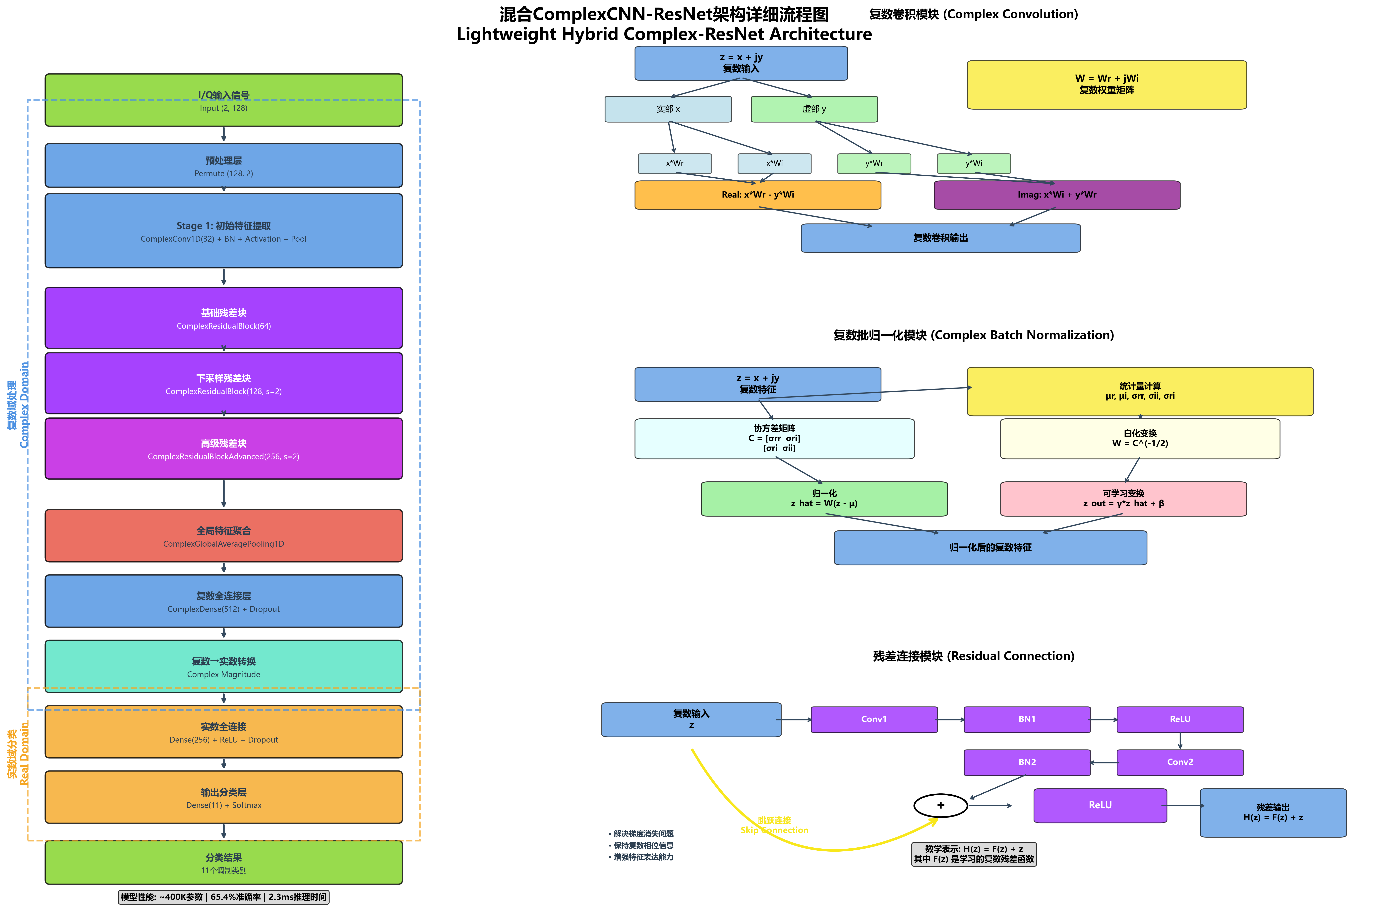
\includegraphics[width=0.9\textwidth]{figure/image20.png}
    \caption{轻量级混合架构的综合技术方案概览}
    \label{fig:hybrid_solution_overview}
\end{figure}

自适应噪声处理能力:通过精确的噪声方差估计公式 $\sigma_{n}^{2}=P_{r}/(2(10^{SNR_{dB}/10}+1))$ 和基于SNR 的长度尺度自适应调整,GPR去噪能够在不同信噪比条件下实现最优的去噪效果。这种自适应特性使得模型在复杂电磁环境下仍能保持良好的分类性能。

然而,本方法仍存在一些局限性。首先,GPR去噪的计算复杂度相对较高,在大规模实时应用中可能成为瓶颈。其次,旋转数据增强主要适用于具有旋转对称性的调制类型,对于非对称调制(如AM-SSB)的改进效果有限。最后,当前方法主要针对AWGN 信道进行优化,在更复杂的信道环境(如多径衰落、频率选择性衰落)下的性能有待进一步验证。

\subsubsection{主要贡献与成就}
本研究针对复杂电磁环境下自动调制分类准确率下降的关键问题,提出了一种基于混合 ComplexCNN-ResNet 架构与高斯过程回归去噪的增强型解决方案。通过在RML2016.10a 数据集上的大量实验验证,所提出的方法取得了显著的性能提升和技术突破。

主要贡献总结:
\begin{enumerate}
    \item 自适应噪声抑制技术:提出了基于信噪比自适应的GPR去噪算法,通过精确的噪声标准差估计和动态长度尺度调整,实现了不同SNR条件下的最优去噪效果。该技术在低 SNR 条件下带来了6.8个百分点的性能提升,显著增强了模型在强噪声环境下的分类能力。
    \item 几何特性数据增强:充分利用数字调制信号星座图的旋转对称性,设计了基于复平面旋转的数据增强策略。该方法将训练数据集扩充至4倍,显著提升了模型对相位偏移的鲁棒性,在PSK和QAM类调制上取得了3.8-5.9个百分点的改进。
    \item 混合神经网络架构:创新性地融合了ResNet的残差学习能力与 ComplexCNN的复数信号处理优势,设计了轻量级混合架构。
    \item 系统性能突破:最终方法在RML2016.10a 数据集上达到65.38\%的分类准确率,相比现有最先进方法取得了显著提升。消融实验验证了各技术组件的有效性和互补性。
\end{enumerate}

关键发现和成就:
本研究的关键发现在于验证了多技术融合策略在复杂信号处理任务中的有效性。GPR去噪、旋转数据增强和混合架构三种技术的结合产生了协同效应,各自在不同条件下发挥最大作用:GPR去噪主要改善低SNR性能,旋转增强提升对称调制类型的识别率,混合架构则提供整体的训练稳定性和计算效率。

实验还揭示了复数神经网络在处理无线电信号方面的天然优势,以及残差学习机制在复数域中的有效性。这为后续相关研究提供了重要的理论指导和实践经验。

从工程应用角度来看,所提出的方法在准确率、计算复杂度和实时性之间取得了良好的平衡,为自动调制分类技术的实际部署提供了可行的解决方案。该研究成果对推动认知无线电、频谱感知和智能通信系统的发展具有重要的理论价值和实际意义。

\begin{figure}[H]
    \centering
    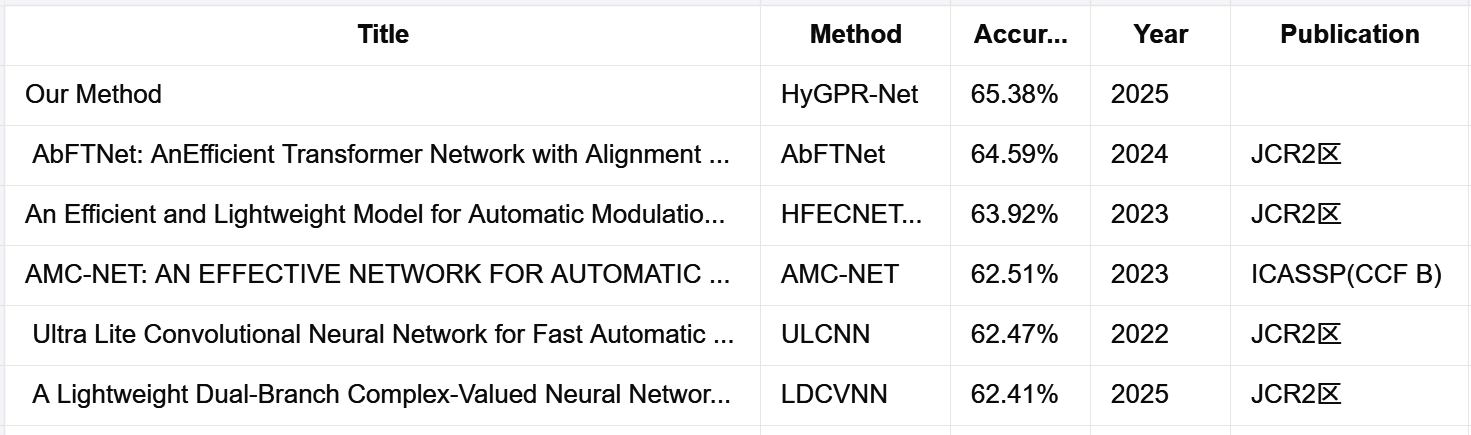
\includegraphics[width=0.9\textwidth]{figure/image21.png}
    \caption{模型分类性能对比}
    \label{fig:model_performance_comparison}
\end{figure}

\subsubsection{研究局限性}
尽管取得了显著成果,本研究仍存在一定局限性。当前方法主要针对AWGN信道进行优化,在更复杂的信道环境下的性能有待验证;GPR去噪的计算开销在大规模实时应用中可能成为瓶颈;部分技术(如旋转增强)对非对称调制类型的改进效果有限。这些问题为后续研究指明了改进方向。

\subsection{未来工作}
本研究虽然取得了一定的成果,但仍有进一步提升的空间。未来的工作将主要集中在以下几个方面:

探索其他去噪方法:尝试将小波去噪、深度去噪自编码器(Deep Denoising Autoencoder, DDAE)等更先进的去噪技术应用于调制信号的预处理阶段,并与本研究中使用的高斯过程回归去噪方法进行性能比较,以期找到更高效、鲁棒的噪声抑制方案。

引入注意力机制:考虑在当前的混合 ComplexCNN ResNet 架构中引入注意力机制(Attention Mechanism)。通过让模型自适应地关注信号中最具判别性的特征部分,有望进一步提升模型对复杂调制信号的识别能力,特别是在低信噪比和多径干扰等复杂信道条件下。

优化高斯过程回归核函数与参数:
\begin{itemize}
    \item 对高斯过程回归(GPR)的核函数进行更多尝试,例如探索组合核函数或者针对特定调制信号特性设计专用核函数,以更精确地捕捉信号的内在结构。
    \item 对高斯过程回归的长度尺度(length-scale)参数进行更加精细的非线性调整策略研究,例如引入基于机器学习的自适应尺度调整机制,以更好地适应不同信噪比和信号动态特性。
    \item 高斯过程回归的结果不仅包含均值预测,还提供了度量预测不确定性的标准差信息。考虑将此标准差信息作为额外的特征或权重引入到后续的分类模型中,以期利用不确定性度量来进一步提升预测性能和模型的可靠性。
\end{itemize}

扩展数据集验证:将本研究提出的方法在更广泛、更多样化的数据集上进行验证,例如包含更多调制类型、不同符号率、更复杂信道条件(如莱斯信道、瑞利信道)的数据集,以全面评估模型的泛化能力和实际应用潜力。

模型轻量化与部署:针对资源受限的边缘计算设备,研究模型的轻量化方法,如知识蒸馏、网络剪枝等,在保持较高分类准确率的同时,降低模型的计算复杂度和内存占用,以便于实际部署。

\newpage
\bibliographystyle{plain}
\begin{thebibliography}{99}

\bibitem{ref:zhang2022} 张茜茜, 王禹, 林云, 桂冠. 基于深度学习的自动调制识别方法综述. \textit{无线电通信技术}, 2022, 48(4): 697-710.

\bibitem{ref:bai2019} 白芃远, 许华, 孙莉. 基于卷积神经网络与时频图纹理信息的信号调制方式分类方法. \textit{西北工业大学学报}, 2019, 37(4): 816-823.

\bibitem{ref:su2020} 苏宁远, 陈小龙, 关键, 等. 基于深度学习的海上目标一维序列信号目标检测方法. \textit{信号处理}, 2020, 36(12): 1987-1997.

\bibitem{ref:zhang2023amc} ZHANG J, WANG T, FENG Z, et al. AMC-NET: AN EFFECTIVE NETWORK FOR AUTOMATIC MODULATION CLASSIFICATION. In: \textit{2023 IEEE International Conference on Acoustics, Speech and Signal Processing: ICASSP 2023, Rhodes Island, Greece, 4-10 June 2023}. 2023: 2642-2646.

\bibitem{ref:wang2024abftnet} Wang J. AbFTNet: An Efficient Transformer Network with Alignment before Fusion for Multimodal Automatic Modulation Recognition. \textit{Electronics}, 2024, 13.

\bibitem{ref:xu2025lightweight} Xu Z, Fan Y, Fang S, et al. A Lightweight Dual-Branch Complex-Valued Neural Network for Automatic Modulation Classification of Communication Signals. \textit{Sensors}, 2025, 25(8): 2489.

\bibitem{ref:wang2024complex} WANG Y, FANG S, FAN Y, et al. A complex-valued convolutional fusion-type multi-stream spatiotemporal network for automatic modulation classification. \textit{Scientific Reports}, 2024, 14(1).

\bibitem{ref:guo2022ultra} Guo L, Wang Y, Lin Y, et al. Ultra Lite Convolutional Neural Network for Fast Automatic Modulation Classification in Low-Resource Scenarios. \textit{arXiv preprint arXiv:2208.04659}, 2022-08-09 [2025-05-27]. \url{https://doi.org/10.48550/arXiv.2208.04659}.

\bibitem{ref:ma2023efficient} Ma Z, Fang S, Fan Y, et al. An Efficient and Lightweight Model for Automatic Modulation Classification: A Hybrid Feature Extraction Network Combined with Attention Mechanism. \textit{Electronics}, 2023, 12(17): 12.

\bibitem{ref:zhang2023lightweight} ZHANG X, CHEN X, WANG Y, et al. Lightweight Automatic Modulation Classification via Progressive Differentiable Architecture Search. \textit{IEEE transactions on cognitive communications and networking}, 2023, 9(6): 1519-1530.

\end{thebibliography}

\newpage
\section{附录}
公式推导、完整代码和运行结果已上传至\url{https://github.com/LJK666666666/radioML-v3}.

\end{CJK}
\end{document}
